\begin{figure}[h!]
    \centering
    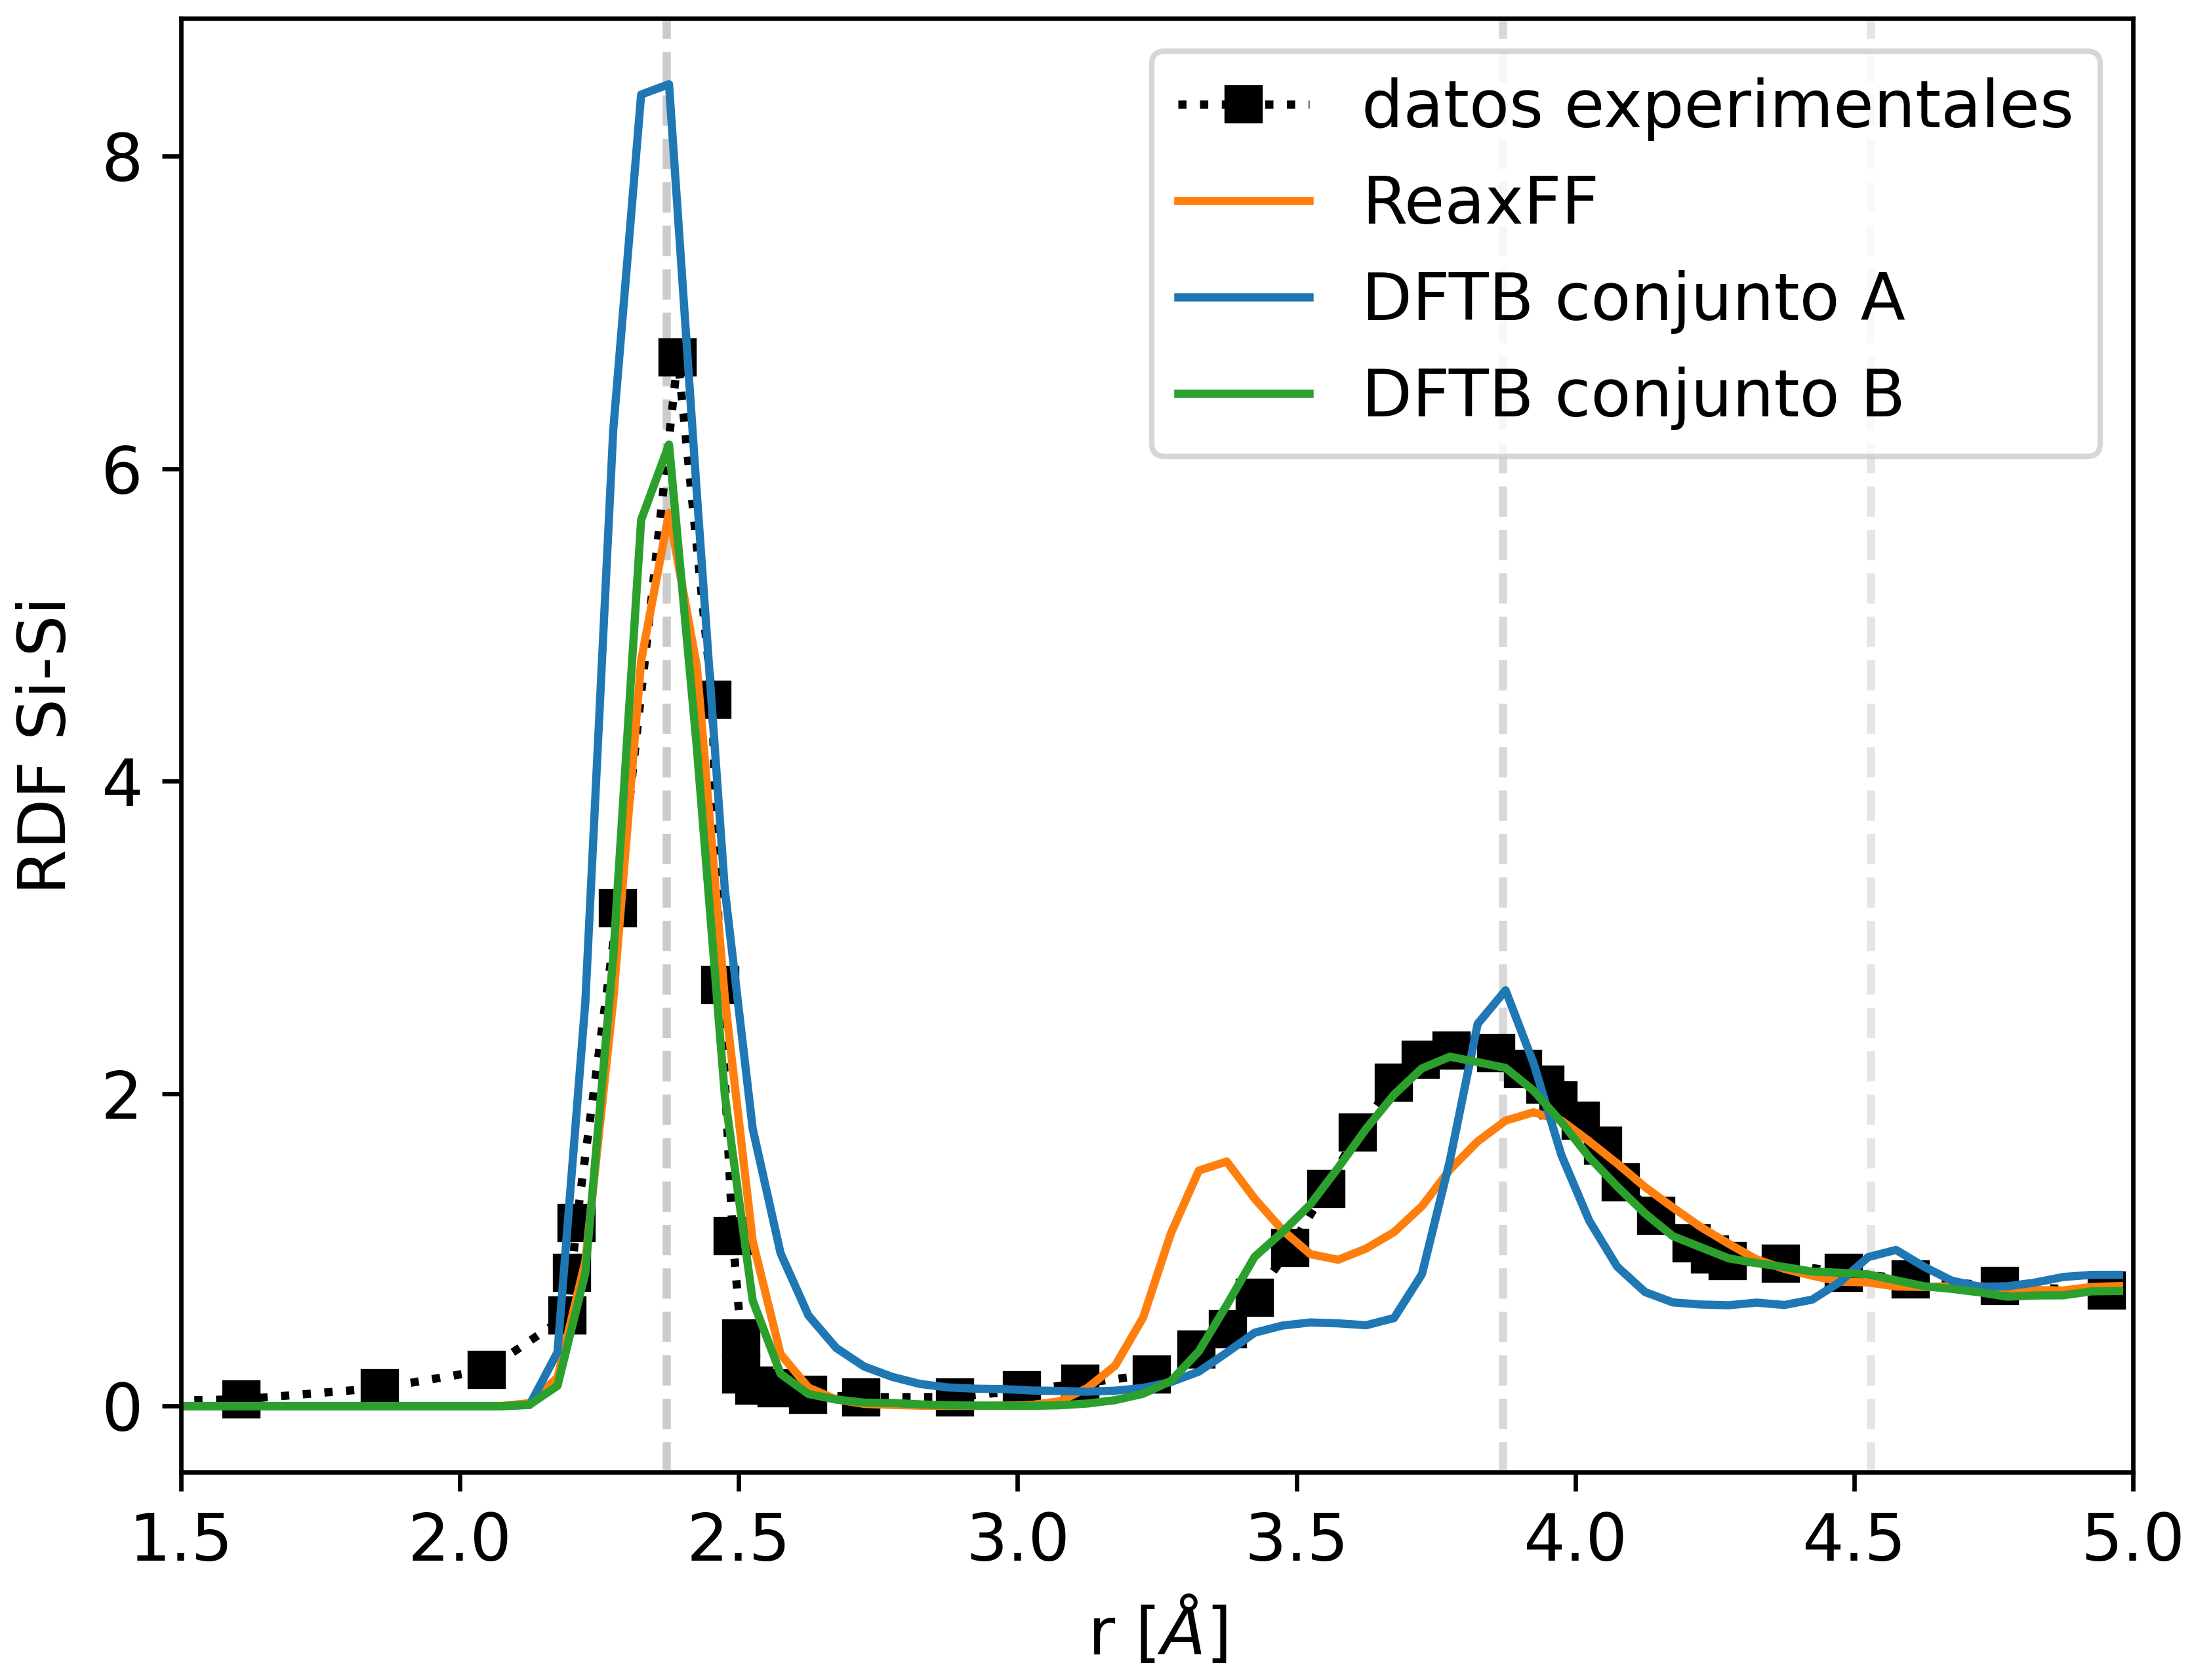
\includegraphics[width=.7\textwidth]{Silicio/modelo/resultados/rdf/rdf.png}
    \caption{Función de distribución radial (RDF) de silicio amorfo para las 
    distintas parametrizaciones de DFTB (A y B). Los resultados se comparan con 
    mediciones referencia TODO y con los resultados del ReaxFF. Las líneas grises 
    discontinuas verticales muestran dónde estarían los picos del silicio 
    cristalino a 0 K. Se encuentra una concordancia excelente entre el experimento
    y la parametrización del conjunto B.}
    \label{fig:rdfb}
\end{figure}
